%--- Heterogeneity by adoption timing relative to the 2010 Maule earthquake
\begin{figure}[h!]
    \centering
    \caption{Effects of \emph{Plan Cuadrante} by Adoption Timing Relative to the 2010 Earthquake}
    \label{fig:heterogeneity_earthquake}
    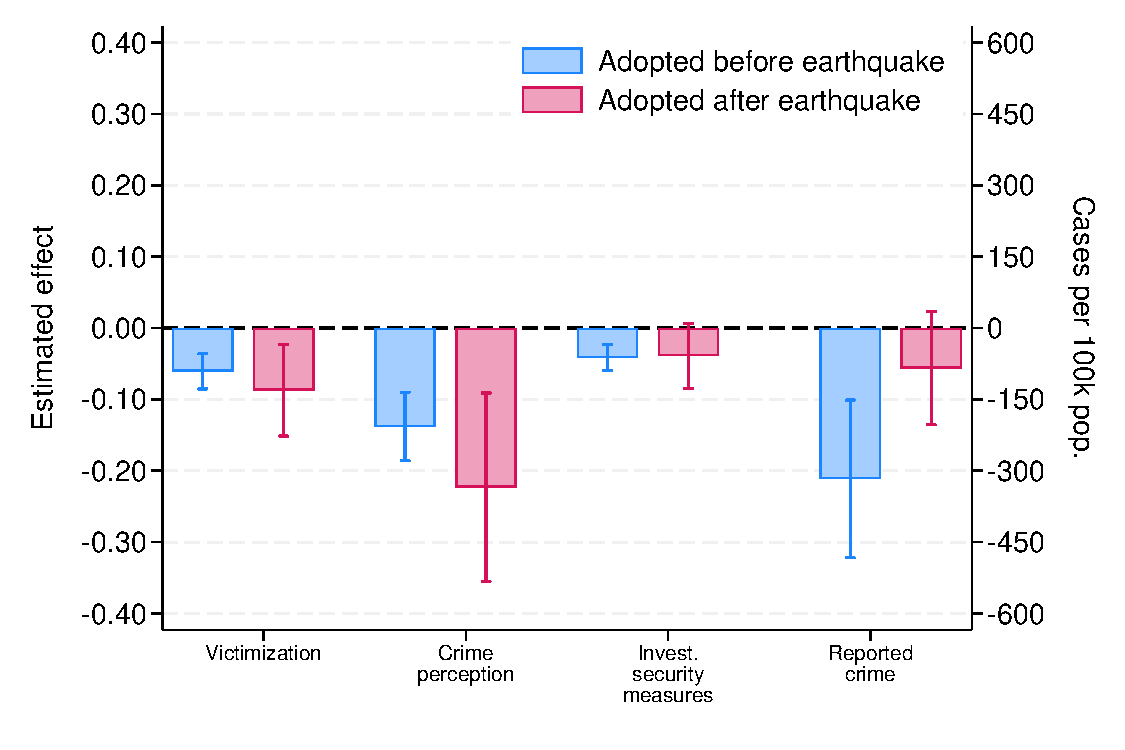
\includegraphics[width=0.8\textwidth]{../manuscript/Graphs/heterogeneity_earthquake.pdf}
    \\[10pt]
    \begin{minipage}{0.99\textwidth}
    \footnotesize
    Notes: This figure exploits the 2010 Maule earthquake (27 February 2010) as a potential source of heterogeneity, comparing the effects of \emph{Plan Cuadrante} for municipalities that adopted the program \emph{before} the earthquake (before 2009, blue bars) and those that adopted it \emph{after} (after 2009, red bars). For each group we estimate the pooled post-treatment effect with the difference-in-differences estimator for staggered adoption of \citet{Callaway}, using never-treated municipalities as controls; the bars represent the average post-treatment effect and the whiskers the 95\% confidence intervals, with standard errors clustered at the municipality level using the wild bootstrapping procedure. Victimization is the probability of household victimization in the last 12 months; crime perception is the probability of perceiving an increase in crime; and investment in security measures is the probability of adopting security measures in the last twelve months---all from the ENUSC survey and read on the left axis. Reported crime is the number of crimes reported to the police per 100,000 inhabitants, from administrative data and read on the right axis.
    \end{minipage}
\end{figure}
